\chapter{Fundamentals II}
\label{cha:Fundamentals II}

This chapter provides an overview of foundational concepts relevant to the thesis. It begins by reviewing various positioning methods as well as systems for indoor and outdoor settings, followed by an examination of how smartphones handle alerts, including different types and influencing factors in iOS. Geofencing technologies are analyzed for their functionality, use cases and limitations. Finally, advancements in technologies such as speech-to-text and large language models are discussed in the context of voice-controlled reminder systems.

\section{Positioning Methods}
The term "positioning" refers to the ability to determine an object's location within a defined space. According to K\"upper \cite{kupper2005location}, positioning relies on the measurement of observables, which describe the spatial relationship between a target and its reference points. Depending on the positioning technology used, observables can include angles, ranges, range differences or velocity and and they are measured by analyzing the properties of pilot signals. 
Pilot signals, such as radio, infrared or ultrasound signals, are reference signals transmitted from a known source and by identifying their origin—a fixed point with known coordinates—the position of the target can be calculated using positioning techniques. These techniques vary based on the type of observable measured and include proximity sensing, lateration, angulation and inertial navigation.
The computed position is expressed relative to a chosen reference system. This system could be descriptive, such as identifying a specific cell in a grid, or geodetic, where the position is represented as two- or three-dimensional coordinates in systems like WGS-84. Further details on the different positioning techniques are provided in the following sections.

\subsection{Proximity Sensing}
Proximity sensing, as described by K\"upper \cite{kupper2005location}, is the most widely used positioning method.
It works by leveraging the limited coverage range of pilot signals to detect the presence or absence of a terminal within a specific area. 
In this context, a terminal refers to a device or object whose position is being determined, such as a mobile or IoT device.
Due to the limited range of these pilot signals, the terminal's position is assumed to correspond to the location of the base station communicating with it.
Militaru et al. \cite{militaru2024positioning} illustrate the concept of proximity sensing in Fig.~\ref{fig:proximity2}.

\begin{figure}[htbp]
    \centering
    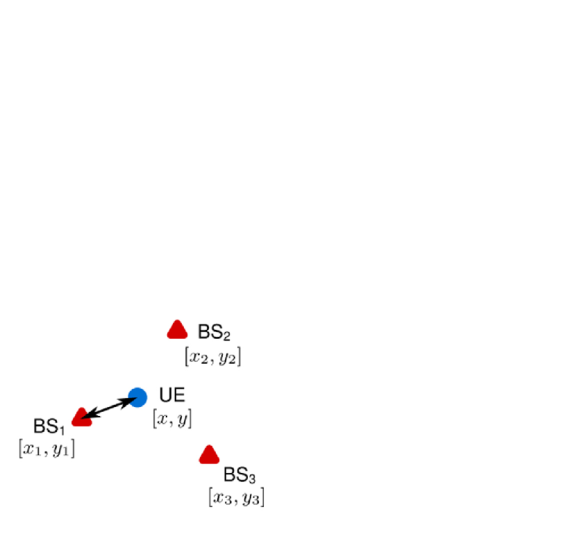
\includegraphics[width=0.4\textwidth]{proximity2.pdf}
    \caption{Proximity sensing \cite{militaru2024positioning}}
    \label{fig:proximity2}
\end{figure}

In the words of K\"upper \cite{kupper2005location}, proximity sensing in cellular networks is often referred to as Cell of Origin (CoO), Cell Global Identity or Cell-ID. 
A "cell" is a geographic area within the cellular network, managed by a base station that serves as a local signal hub for devices within that area. 
The accuracy of the location determined through CoO depends largely on the size and shape of the cell, as highlighted by Grejner-Brzezinska and Kealy \cite{grejner2004positioning}. 
Smaller cells allow for better location estimates, often reaching accuracy within 100 meters in urban areas where cell towers are densely placed. 
In rural areas, where cell coverage spans several kilometers, the location estimate becomes less accurate.
CoO is commonly used in scenarios where approximate location data is sufficient, such as in emergency services to locate callers or for network optimization by telecom providers. According to Grejner-Brzezinska and Kealy \cite{grejner2004positioning}, CoO is a power-efficient solution, requiring only a single connection to the cell tower. This makes it accessible across cellular networks, even in low-power settings where more intensive GPS tracking may not be feasible.

\subsection{Lateration}
\subsection{Angulation}
Angulation is a positioning technique that determines an object's location based on the angles at which signals are received from multiple reference points, rather than measuring distances. According to K\"upper \cite{kupper2005location} it is also called Angle of Arrival (AoA) or Direction of Arrival (DoA). Werner \cite{werner2014indoor} explains that by using directional antennas or other angle-measuring equipment, the system identifies the direction of incoming signals from known base stations or access points. Once the angles from at least two base stations are known, the object's position can be triangulated by drawing lines along these angles, the point where the lines intersect reveals the target's location, as shown in Fig.~\ref{fig:angulation2}.

\begin{figure}[htbp]
    \centering
    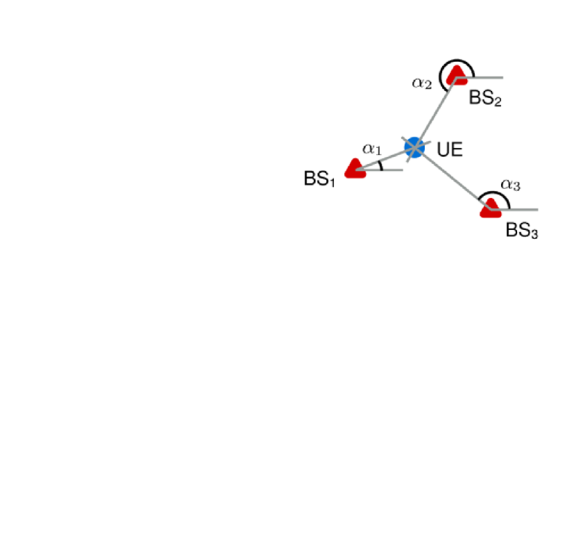
\includegraphics[width=0.4\textwidth]{angulation2.pdf}
    \caption{Triangulation \cite{militaru2024positioning}}
    \label{fig:angulation2}
\end{figure}

In three-dimensional space, a third angle may be required for accurate positioning. Angulation offers an effective alternative to lateration methods, particularly in environments where measuring precise distances is challenging due to signal reflections or interference. However, it does require precise angle measurements, which can be sensitive to minor errors in directionality, especially at long distances.

\subsection{Pattern Matching}
\subsection{Inertial Navigation}

\section{Positioning Systems}
\subsection{Cellular Positioning}
\subsection{GNSS}
%winters2008travel
%The GPS system is a constellation of 24 satellites that broadcast data that can be processed by end-user devices to calculate their position using the Time of Arrival (TOA) method and applying circular lateration in combination with timing measurements. The constellation consists of six orbits spaced 60 degrees apart, with four satellites per orbit. This guarantees that a GPS receiver is under the coverage of at least four satellites at any given point in the earth’s surface.
%since the GPS transmissions from the satellites are very weak, the device must have a clear view of the sky to receive the transmissions used to calculate its position. This means that pure GPS positioning solutions do not work indoors or in situations where radio signals may be interrupted, such as during severe weather or in “urban canyons” (areas surrounded by many tall buildings)

\subsection{WLAN and Bluetooth Positioning}
% \subsection{Sensor-Based Systems}
\subsection{Hybrid Systems}
